\section{Mamdani Fuzzy Inference System}\label{sec:fuzzymamdani}

The Mamdani FIS is available in \code{src/mamdani.fis}. It can be opened with
MATLAB's Fuzzy Logic Designer.

To design the system, I've started by analyzing the distribution of the
features for the three classes. \figref{fig:featdistribhist} shows the
histograms for the 3 features where each color is a different class\footnote{In
the \code{figures} folder, you can also find the histograms divided for each
class, instead of having all classes in a single histogram.}. These histograms
are generated with the script \code{plotfeatdistrib.m}.

\begin{figure}[htbp]
	\centering
	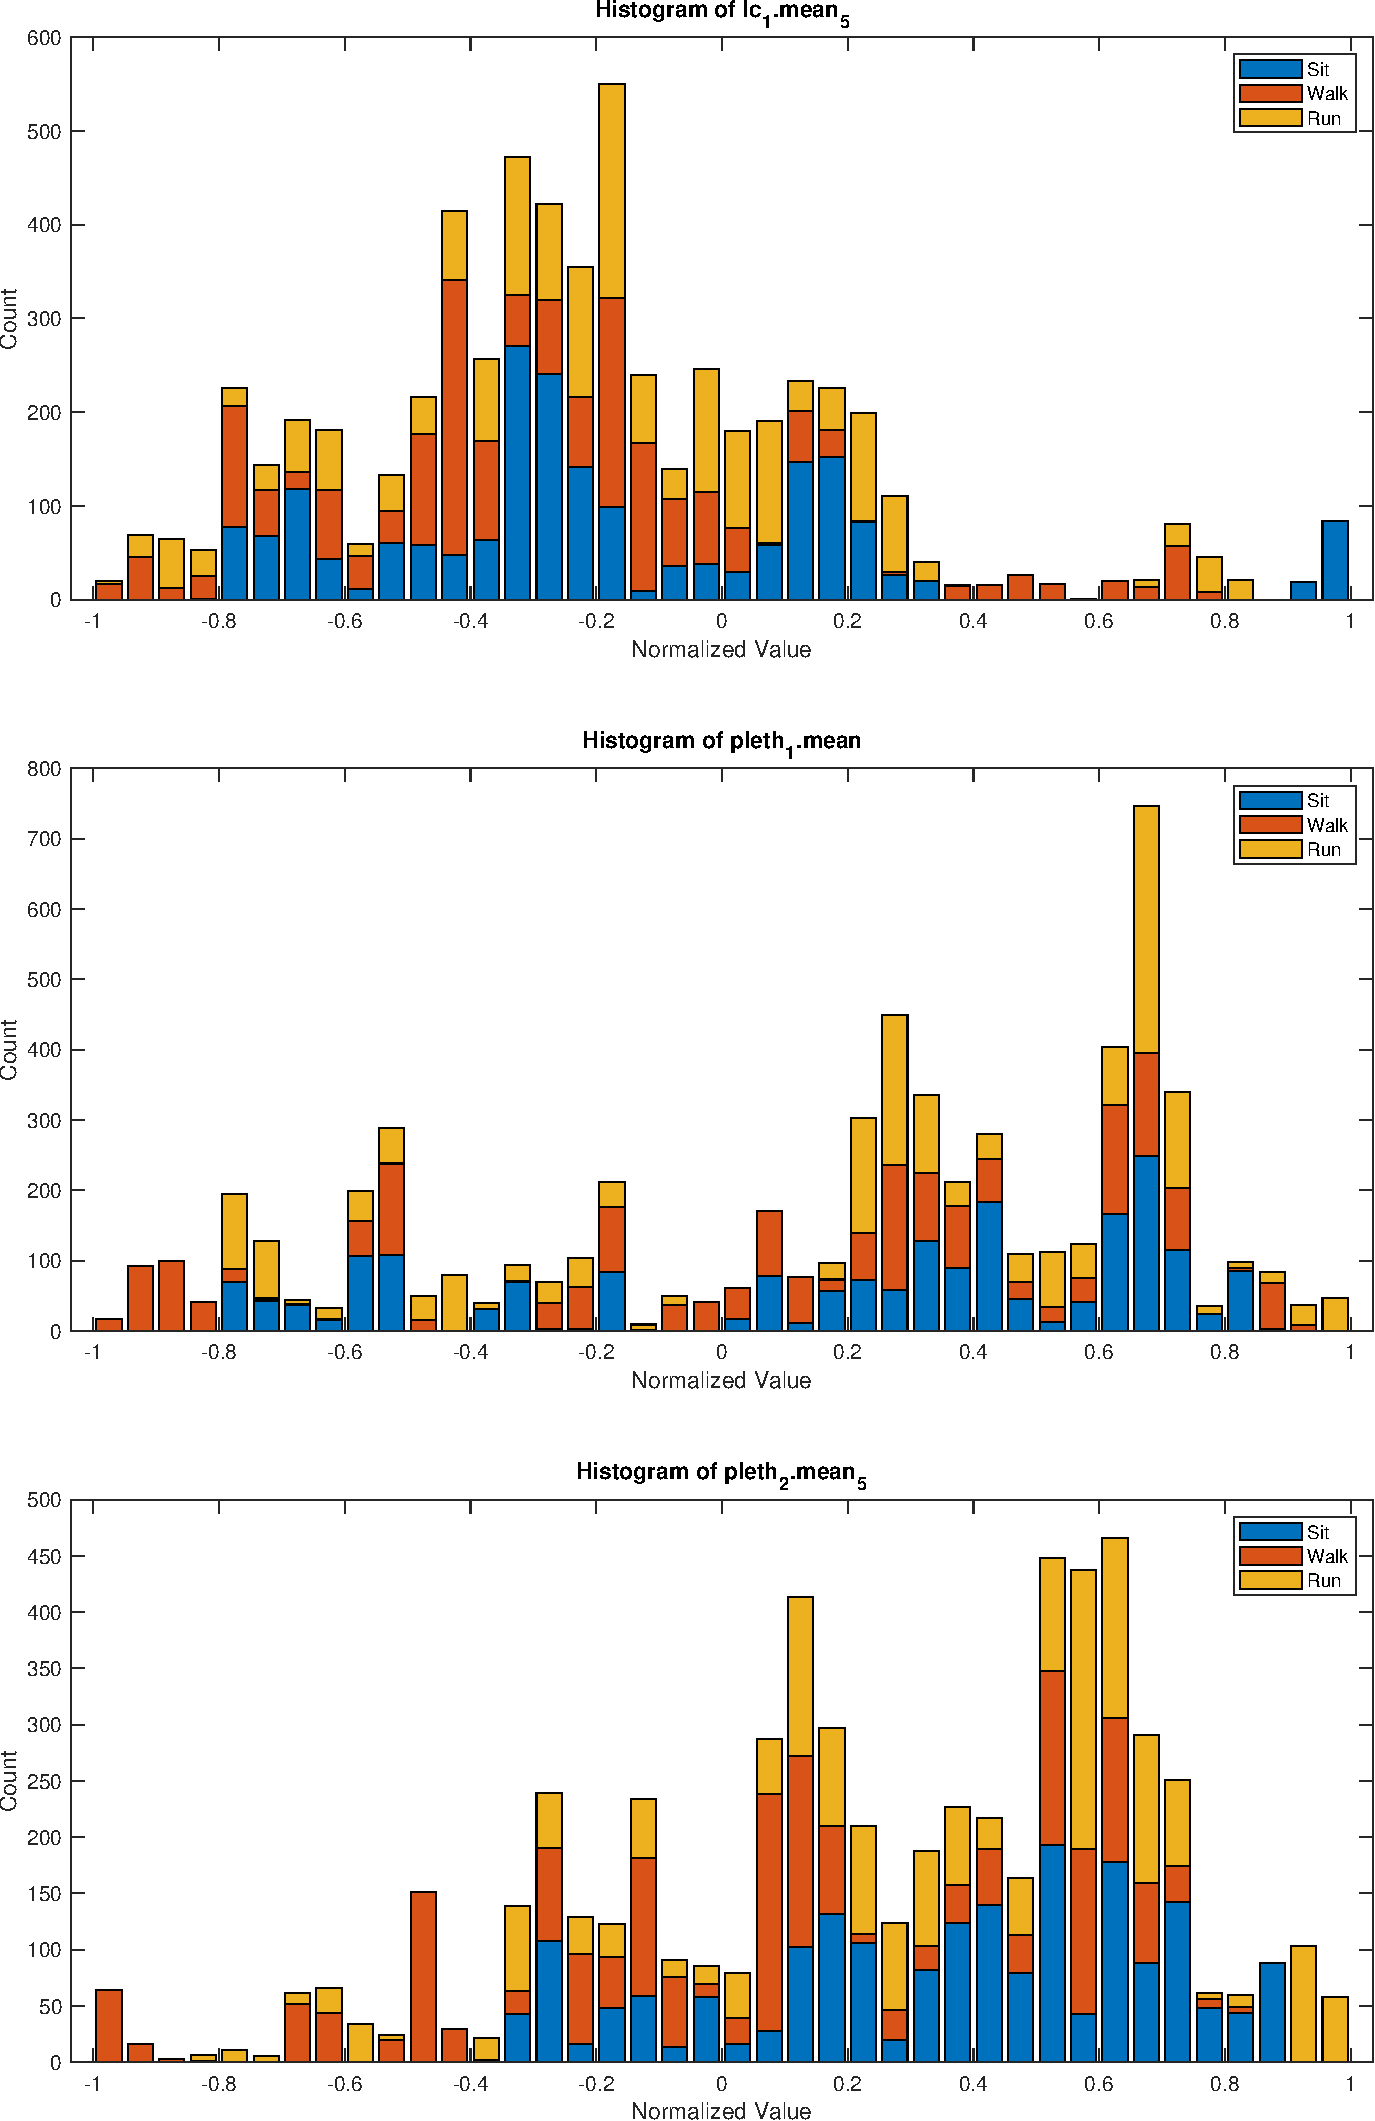
\includegraphics[width=\textwidth]{featdistribhist}
	\caption{Histograms of the distributions of the three features for the
	three classes.}\label{fig:featdistribhist}
\end{figure}

Distributions are skewed: the first attempt was to model the input variables of
the FIS using 4 generalized bell membership functions, by trying to
``condensate'' them more where the feature's distribution is more ``dense''.

Initially, the output variable was modeled as three triangular equal-spaced MFs
with centers in 0 (sit), 1 (walk) and 2 (run), with some degree of overlap.

I've then used the script \code{wangmendel.m} to try to guide the definition of
the rules using an approach I've derived from the Wang-Mendel method. The
script, quite complex, performs the following steps:
\begin{enumerate}
	\item Create a matrix where each row represent a possible rule (any
		combination of the inputs, using \code{AND} or \code{OR} as
		conjuctions). The matrix is pre-filled with all possible rules.
	\item For each sample, compute the membership degree of its features to
		the MFs designed for the FIS.
	\item For each rule, compute the number of samples that would be
		correctly/wrongly classified if the rule is included in the
		FIS. These values are weighted using the membership degree of
		the features of the sample used in the rule under evaluation.
		Like in the ``product strategy'' of the Wang-Mendel method.
	\item To determine the ``importance'' of the rule, the weighted number
		of correctly classified samples is divided by the weighted
		number of uncorrectly-plus-correctly classified
		samples\footnote{Actually, if the misclassified sample is ``far
		away'' from the correct class \idest{correct class is
		\code{sit}, but the rule includes a sample of class \code{run},
		or vice versa}, its weight is doubled. This is done to penalize
		rules that make the FIS confuse between \code{sit} and
		\code{run}.} in order to obtain a (weighted) ratio which
		represents how many samples are correctly classified by the
		rule.
	\item Rules with the above ratio below \(0.5\) are excluded.
	\item That ratio is then rescaled between 0 and 1. It will represent
		the final weight of the rule.
	\item Conflicting rules \idest{same \code{IF} part, different
		\code{THEN} part} are removed, keeping only the rule with the
		highest weights.
	\item Finally, rules are printed on screen, in human readable format
		\idest{``IF \ldots THEN \ldots''}, along with their weight.
\end{enumerate}

I've then added the rules to the Mamdani FIS. Then, since it performed very
poorly, I've started to modify the MFs for the inputs and the output, following
a trial-and-error approach. After defining the new MFs for the inputs, I've
also re-run the \code{wangmendel} script to generate new rules, based on the
new MFs. During this work, I've also removed some rules and changed the weights
of some other rules from the final system. I'll show the final design in the
following sections.

\subsection{Inputs' membership functions}

To optimize inputs' MFs, I've tried to plot in a 3 dimensional space the
samples' classes using \code{plotfeatdistrib} script. This is shown in
\figref{fig:classes3d}.

\begin{figure}[htbp]
	\centering
	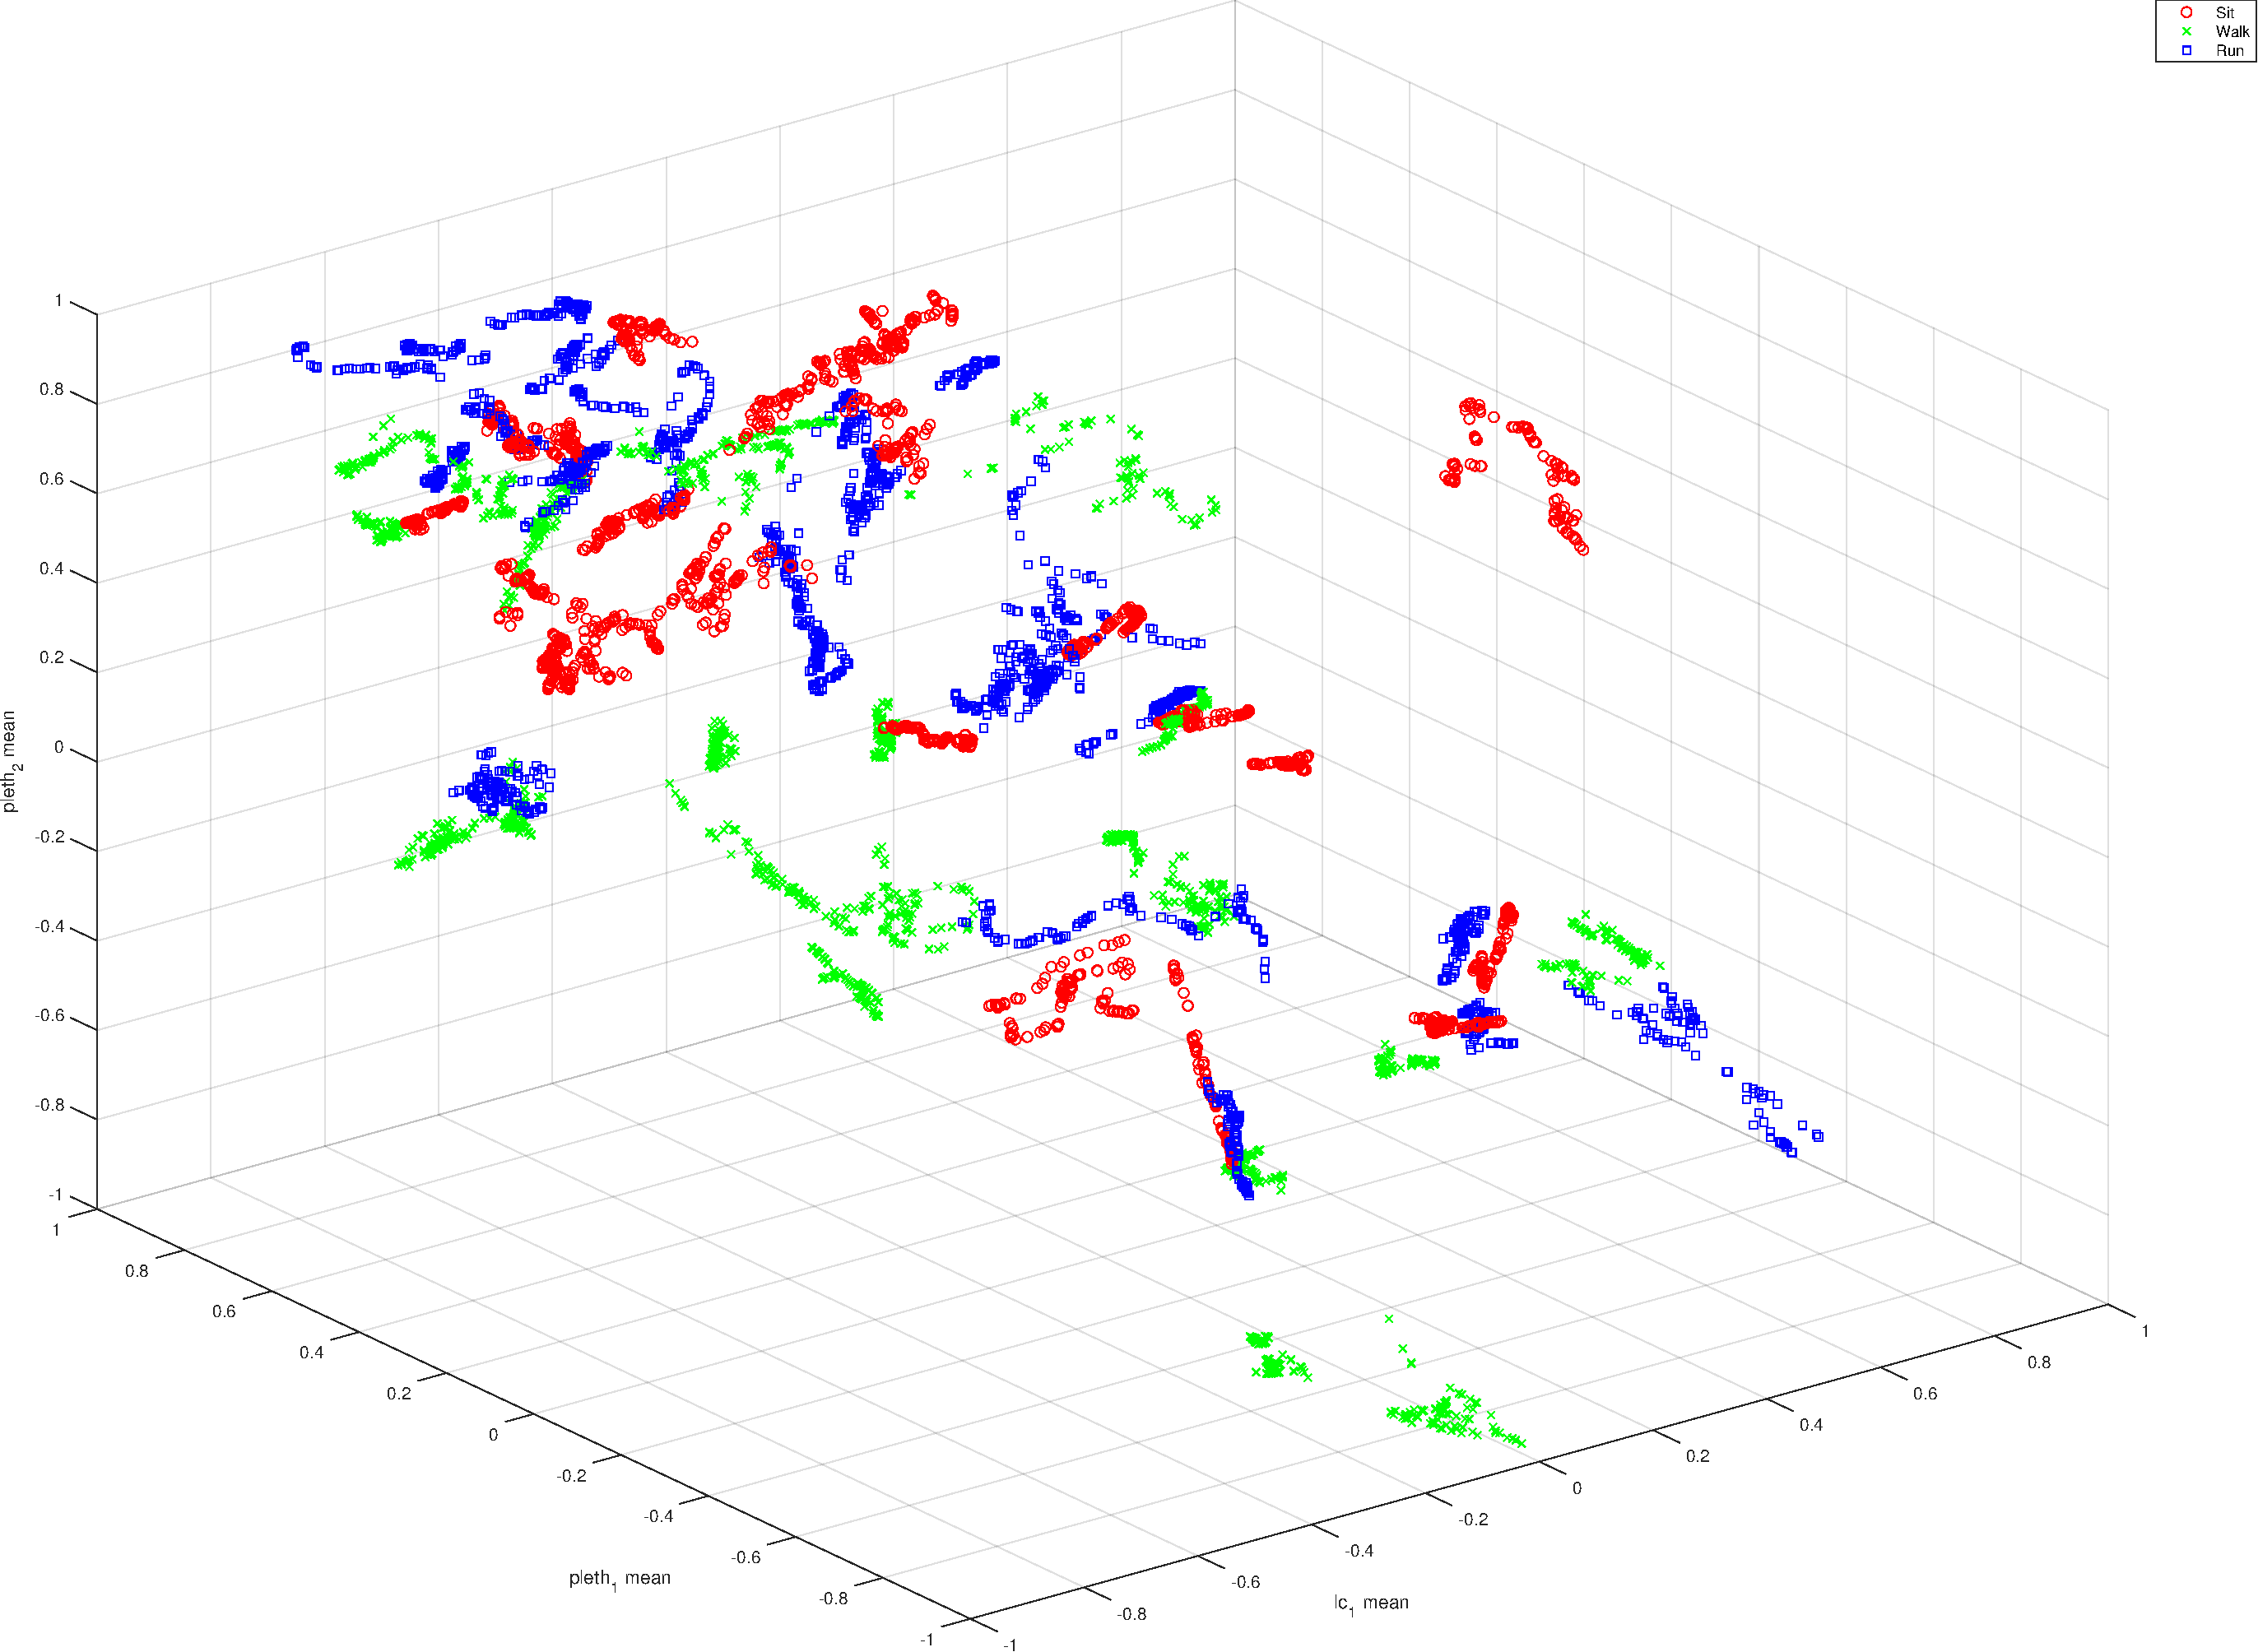
\includegraphics[width=\textwidth]{classes3d}
	\caption{3D plot of all the samples with the normalized features in the
	three axes. Each color is a different class.}\label{fig:classes3d}
\end{figure}

It may be not very clear from the figure in this document, but all the classes
are in \emph{well defined clusters} (it can be seen by rotating the figure in
the MATLAB's window). The problem is that they are in \emph{very small}
clusters. I've tried to manually define hyperboxes for these clusters but I've
gave up when I've realized that, to define these hyperboxes, I would have
needed more than 10 MFs per feature.

So, using a trial-and-error aprroach, I've tried to define 4 generalized bell
MFs for each input. \figref{fig:pleth1meanmfs} shows the MFs defined for the
\code{pleth\_1:mean} feature. The MFs for the other inputs can be seen by
opening \code{mamdani.fis} in the Fuzzy Logic Designer tool, I will not report
them here to save space: they are still generalized bell functions, just moved
around and with different slopes.

\begin{figure}[htbp]
	\centering
	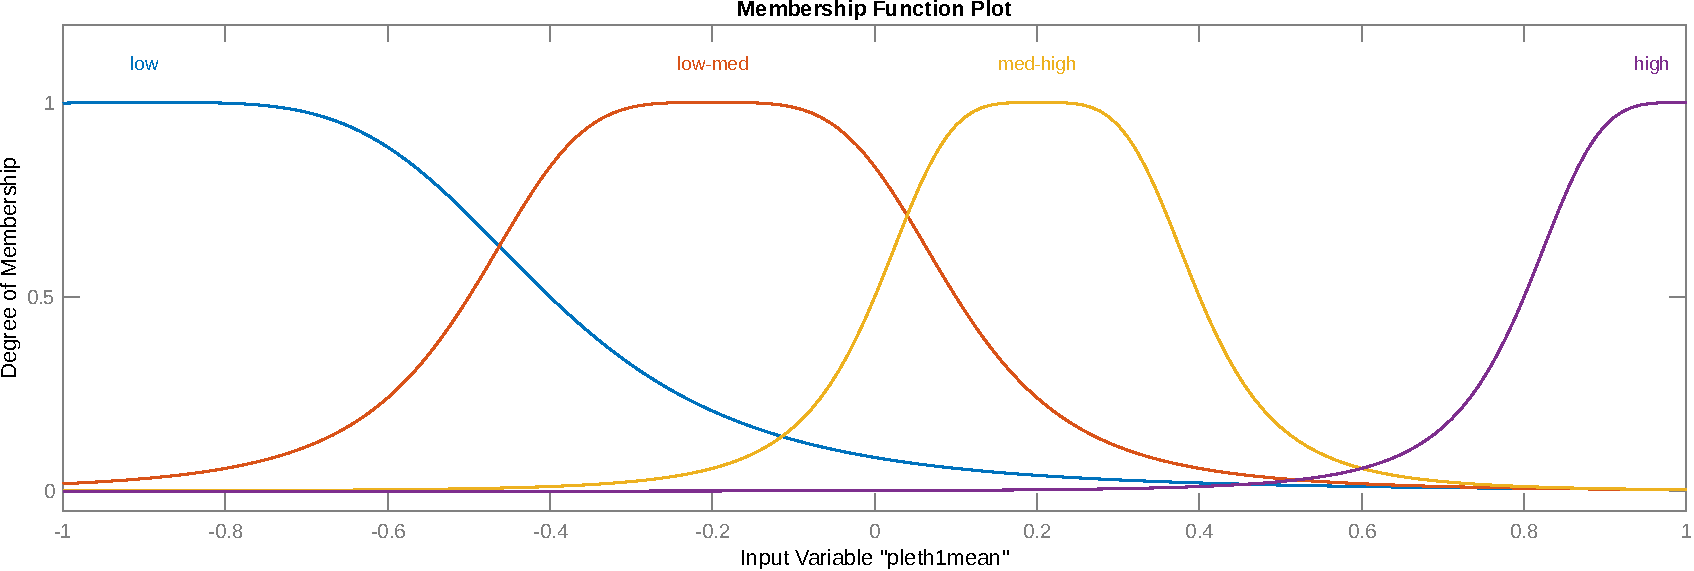
\includegraphics[width=\textwidth]{pleth1meanmfs}
	\caption{Membership functions for
	\code{pleth\_1:mean}.}\label{fig:pleth1meanmfs}
\end{figure}

\subsection{Output's membership functions}

After some tests, I've abandoned the triangular MFs for the output and
switched to sigmoid MFs for the \code{sit} and \code{run} classes and a
generalized bell for the \code{walk} class. I've chosen these MFs since I've
found they were able to reduce an issues I've faced with the FIS: it tends to
favor the class placed in the middle \idest{the \code{walk} class}.
\figref{fig:outputmfs} shows the MFs for the output variable.

\begin{figure}[htbp]
	\centering
	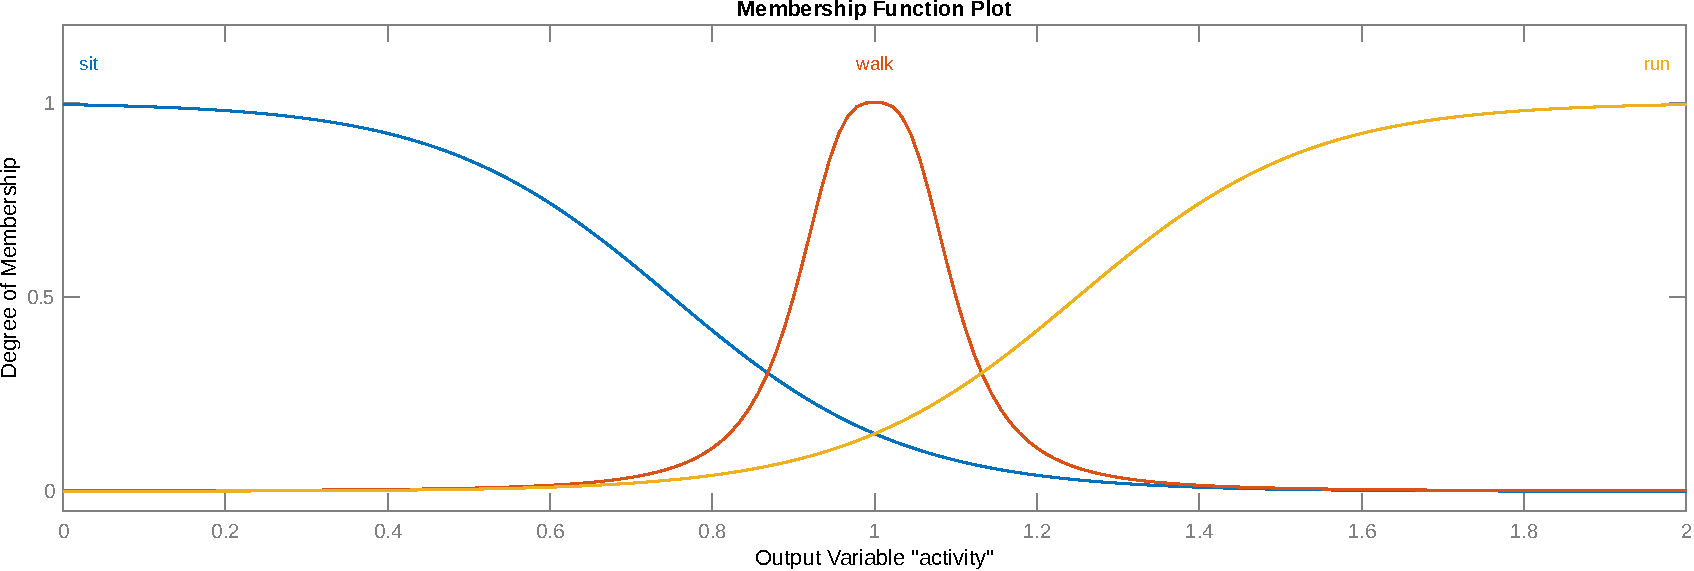
\includegraphics[width=\textwidth]{outputmfs}
	\caption{Membership functions for the output.}\label{fig:outputmfs}
\end{figure}

\subsection{Rules}

As said, rules are defined using the \code{wangmendel.m} script. Then, by
trial-and-error, I've removed some rules and changed the weight of others. The
final set of rules used is shown in \figref{fig:mamdanirules}.

\begin{figure}[htbp]
	\centering
	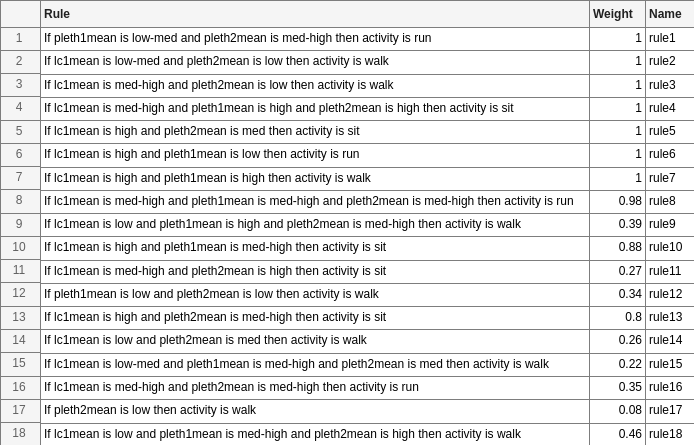
\includegraphics[width=\textwidth]{mamdanirules}
	\caption{Mamdani rules with their weights.}\label{fig:mamdanirules}
\end{figure}

\subsection{System configuration}

With ``system configuration'' I mean the methods used to perform the \code{AND}
and \code{OR} operations, the implication and aggregation methods, and the
defuzzification method. I've tried all possible combinations of these
parameters. The ones that yielded the best results are shown in
\tableref{table:mamdaniconfig}.

\begin{table}[hbtp]
	\centering
	\begin{tabular}{|r|c|}
		\toprule
		Parameter name & Chosen method \\
		\midrule
		\code{AND} method & \code{prod} \\
		\code{OR} method & \code{max} \\
		Implication method & \code{min} \\
		Aggregation method & \code{max} \\
		Defuzzification method & \code{MOM} \\
		\bottomrule
	\end{tabular}
	\caption{Best system configuration for the Mamdani
	FIS.}\label{table:mamdaniconfig}
\end{table}

I will note that the \code{centroid} method was inadequate since it was making
the FIS to classify nearly all the samples as \code{walk}: since it is the
central MF for the output, when the FIS was undecided between \code{sit} and
\code{run}, it was outputting \code{walk} with very high membership degree. It
may be fine for a FIS, if you think that ``sit'' should be read as ``not
moving'', ``walk'' should be read as ``moving slowly'' and ``run'' should be
read as ``moving fast'': the \code{walk} class can represent the undecision
between \code{sit} and \code{run}. But the system, with the \code{centroid}
method, was unable to correctly classify samples of the \code{sit} and
\code{run} activities.

As a final note, a possible solution for the preference of the FIS for the
\code{walk} class may be to split the output space into 3 different outputs,
each with a single membership function which represent the confidence level
that the FIS has in the class. I've not tested this approach anyway.

\subsection{Results}

Confusion matrix generated by script \code{mamdanitest.m} is shown in
\figref{fig:mamdaniconfusion} (output of the FIS is considered as the class
with the highest membership degree). Note that the system still classifies most
samples as \code{walk}. Performances are poor: less than half of the samples
are correctly classified. I was unable to get any better. Probably a type-1
Mamdani FIS with only 4 MFs per input is too simple for this task. In
\secref{sec:fuzzyanfis}, I've developed another FIS which perfomed very well.

\begin{figure}[htbp]
	\centering
	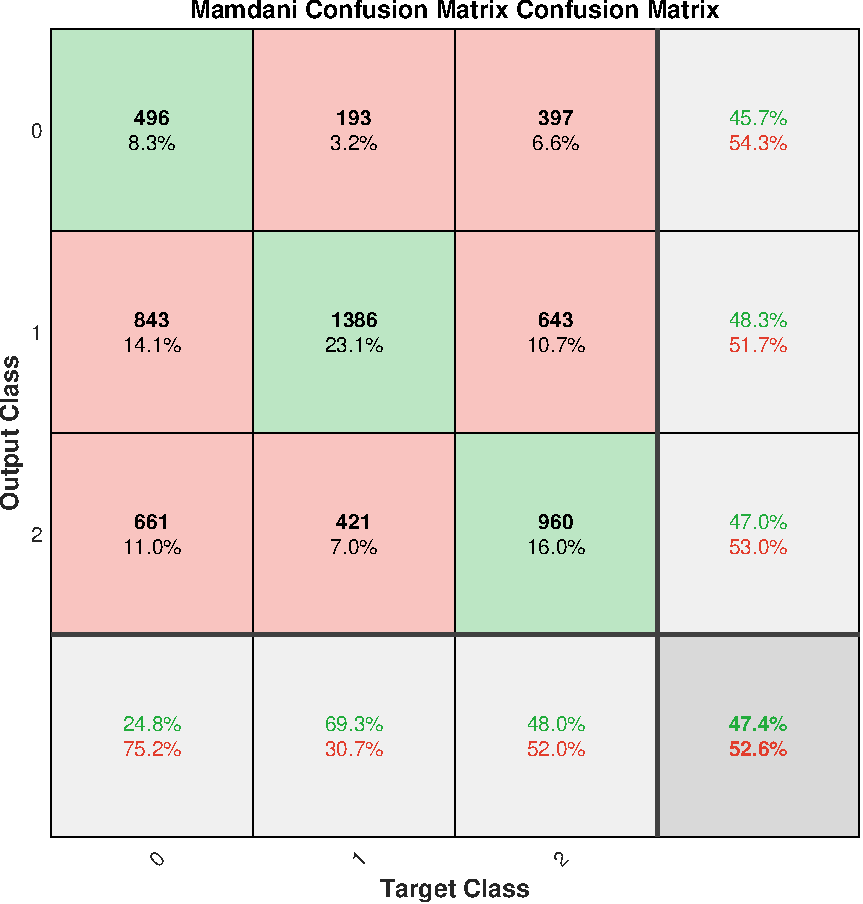
\includegraphics[width=0.6\textwidth]{mamdaniconfusion}
	\caption{The confusion matrix for the Mamdani system shows poor
	performances and a preference for the \code{walk}
	class.}\label{fig:mamdaniconfusion}
\end{figure}
